\section{Vector Algebra}
\begin{figure}[H]
	\centering
	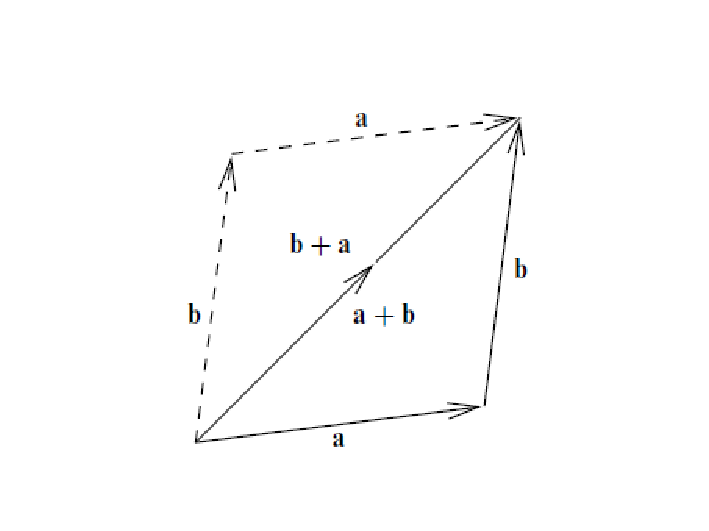
\includegraphics[scale=1]{figures/vector_add.pdf}
	\caption{\label{vector_add} Addition of two vectors using Parallelogram Law}
\end{figure}
\subsection{Scalar Product}
\begin{defn}[Dot Product]
For two vectors $a$ and $b$, the scalar product, or the dot product, is defined as:
\begin{align*}
a \cdot b &= \lvert a \rvert \lvert b \rvert \cos\theta \\
&= \langle a |b \rangle
\end{align*}
Where $\theta$ is the angle between the two vectors.
\end{defn}
If $a = x_1 \hat{\imath} + y_1 \hat{\jmath} + z_1 \hat{k}$ and $b = x_2 \hat{\imath} + y_2 \hat{\jmath} + z_2 \hat{k}$ then,
$$a \cdot b = (x_1 x_2)\hat{\imath} + (y_1 y_2)\hat{\jmath} + (z_1 z_2)\hat{k}$$
If $a \perp b$, then $a\cdot b = 0$ and, if $a \parallel b$, then $a\cdot b = |a||b|$

\subsection{Vector Product}
\begin{defn}[Cross Product]
For two vectors $a$ and $b$, the vector product, or the cross product, is defined as:
\begin{align*}
a\times b &= \lvert a \rvert \lvert b \rvert \sin\theta \\
&=|b\rangle \langle a|
\end{align*}
Where $\theta$ is the angle between the two vectors.
\end{defn}
If $a = x_1 \hat{\imath} + y_1 \hat{\jmath} + z_1 \hat{k}$ and $b = x_2 \hat{\imath} + y_2 \hat{\jmath} + z_2 \hat{k}$ then,
$$
a \times b =
\begin{vmatrix}
\hat{\imath} & \hat{\jmath} & \hat{k} \\
x_1 & y_1 & z_1 \\
x_2 & y_2 & z_2 \\
\end{vmatrix}
$$
The resultant is a vector $a\times{b}$ that is mutually perpendicular to both, $a$ and $b$.
\subsection{Triple Products}
\paragraph{Scalar Triple Product}
$$[a\  b\  c] = (a\times b)\cdot c = a\cdot(b\times c) = \begin{vmatrix}
a_1 & a_2 & a_3 \\
b_1 & b_2 & b_3 \\
c_1 & c_2 & c_3
\end{vmatrix}$$
\subsection{Equations of lines, planes and spheres}

\paragraph{Equation of a line}
In Fig.\ref{eqnline}, the vector {\bfseries r} can be written as $\mathbf{r} = \mathbf{a + \lambda b}$
\begin{figure}[H]
	\centering
	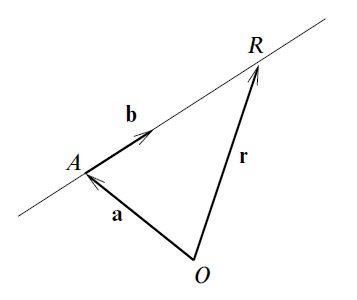
\includegraphics[scale=0.75]{figures/line}
	\caption{\label{eqnline} The equation of a line. The vector b is in the direction \emph{AR} and $\mathcal{\lambda}$b is the vector from \emph{A} to \emph{R}.}
\end{figure}
General Equation of a line:
$$\frac{x-x_1}{a} = \frac{y- y_1}{b} = \frac{z-z_1}{c}$$

Parametric Equation of a line:
\begin{align*}
	&x = x_1 + at & &y= y_1 +bt & &z= z_1 +ct
\end{align*}

Where $t$ is a parameter
\paragraph{Equation of a Plane}

